\chapter{Suggested Future Research}
\section{Continuation of Exposures and Analysis}


%%%%%%%%%%%%%%%%%%%%%%%%%%%%%%%%%%%%%%%%%%%
\subsection{Improvement}
There are at least two aspects we can improve in the next stage,

\begin{enumerate}

    \item \textbf{More Detailed Action Space}: Here only three actions are defined and the car is always in acceleration mode which is not the best choice in some cases. When the car is got stuck, acceleration wastes the effort of getting out. And it is easier to pass the sharp turn if it slows down the speed a little bit. Thus we can define more actions as follows.
	\begin{figure}[h]
	\centering
	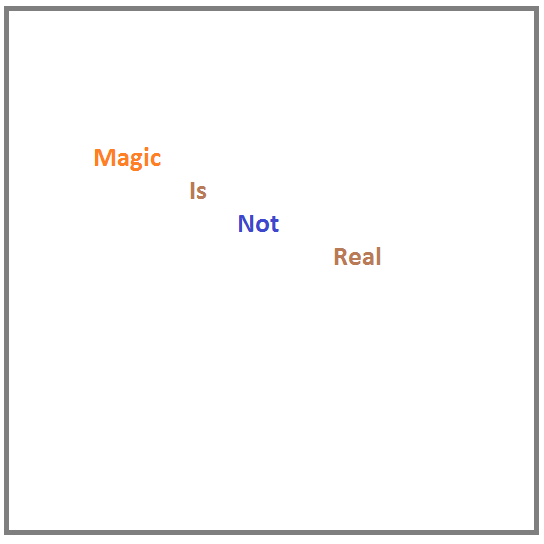
\includegraphics[width=0.5\textwidth]{figs/magic}
	\caption{A bigger action space.}
	\end{figure}    
    
    \item \textbf{Tuned Reward Functions:} In this project, I almost relied on the game score as the reward resource. In fact, there are some rules to get maximal rewards which I don't think help learning a reasonable driving behavior. For example, there is no punishment on being blocked and falling into the sky. The Game Bot may think it is no big deal to fall into the sky and sometimes it can be rewarded 1000 score if it happen to hit a traffic cone before it falls down. I put my focus on building a working Deep Q Learning structure and had a hard time hacking into the scoring system, so I have to put this task next time.
    \item \textbf{Better benchmarks:} In most of this project we used simple benchmarks, such as playing against random players. While testing against random is probably the first thing to test against (if you can't beat a random player your learning algorithm is not working), it would be better to find a few heuristics and better players that can be used for testing.

    \item \textbf{Incorporate other RL techniques:} The field of RL has been advancing fast in recent years. There are a few new and old techniques that I would like to try, such as asynchronous RL, double Q-learning, prioritized experience replay and Asynchronous Actor-Critic Agents (A3C).

\end{enumerate}
